\documentclass{article}
\usepackage{lmodern}
\usepackage[francais]{babel}
\usepackage[utf8]{inputenc}
\usepackage{graphicx}
\usepackage{shortvrb}
\usepackage{amssymb}
\usepackage{amsmath}
\usepackage{listings}
\usepackage{mathtools}

\title{TIPE: Introduction à la théorie des ondelettes}
\author{Xavier Friederich et Gaétan Bahl}

\begin{document}
\maketitle
\tableofcontents
\listoffigures
\MakeShortVerb{@}
\clearpage

\newcommand{\fonction}[5]{\begin{array}{l|rcl}
#1: & #2 & \longrightarrow & #3 \\
    & #4 & \longmapsto & #5 \end{array}}

\section{Premières définitions}


La transformation en ondelettes est apparue pour la première fois dans le domaine de la géophysique vers 1980 pour l’analyse des données sismiques. Elle aura été formalisée par Morlet, Grassmann et Goupillard.
De manière analogue à la théorie des séries de Fourier, les ondelettes sont principalement utilisées pour la décomposition de fonctions. La décomposition d’une fonction en ondelettes consiste à l’écrire comme une somme pondérée de fonctions obtenues à partir d’opérations simples effectuées sur une fonction principale appelée ondelette-mère. Ces opérations consistent en des translations et dilatations de la variable. Selon que ces translations et dilatations sont choisies de manière continue ou discrète, on parlera d’une transformée en ondelettes discrète ou continue.
Le travail suivant fera l’objet du cas particulier de la transformation en ondelettes unidimensionnelle.



\subsection{Définition 1 : Ondelette}

Une ondelette est d’un point de vue géométrique et schématique une forme d’onde, l’idéalisation d’une note de musique, d’une durée limitée et qui a une valeur moyenne égale à 0. 

Plus formellement, pour le cas d’une ondelette-mère (celle que l’on va pouvoir dilater et translater afin d’obtenir les autres ondelettes définissant ainsi une famille d’ondelettes), il s’agit d’une fonction $\psi$ de l'espace de Lebesgue $L^2(\mathbb{R}$) (espace des fonctions à valeurs dans $\mathbb{C}$ de carré intégrable) et telle que :

$\int_{\mathbb{R}}\psi{}(t)\cdot{}dt = 0$

ce qui provient de la condition $\int_{\mathbb{R}} \frac{|\hat{\psi}(\omega)|^2}{|\omega|}d\omega < \infty$ où $\hat{\psi}$ est la transformée de Fourier de $\psi$, donnée par la formule $\displaystyle \hat{\psi}(\omega)= \int_{-\infty}^{+\infty}\psi{}(t)\cdot{}e^{-2i\pi\omega{}t}dt$

Cette condition, dite condition d’admissibilité est nécessaire pour que la transformée en ondelettes d’une fonction existe !

Si l'ondelette -fonction analysante- est convenablement choisie, la transformation en ondelettes est inversible et la fonction peut être reconstruite après analyse suivant l'équation : \\

$\displaystyle f = C_{\psi}^{-1}\int_{-\infty}^{+\infty}\int_{-\infty}^{+\infty}\frac{1}{a^2}\langle{}f,\psi{}_{a,b}\rangle\psi{a,b}da\cdot{}db$ \\


Le coefficient $C_{\psi}$, si donc il existe, est donné par : $\displaystyle C_{\psi} = 2\pi\int_{\mathbb{R}}\frac{|\hat{\psi{}(\omega)}|^2}{|\omega|}d\omega < \infty$


De manière plus << imagée >>, l’ondelette doit osciller localement autour de l’axe des abscisses.
Il existe une infinité de fonctions d’ondelettes car toute fonction oscillante localisée est une ondelette-mère possible.
Différentes familles d’ondelettes peuvent être utilisées en fonction du problème à résoudre. C’est un des nombreux avantages de la transformée en ondelettes par rapport à la transformée de Fourier (qui est liée exclusivement aux fonctions sinus et cosinus) que de pouvoir choisir l’ondelette à utiliser pour l’analyse.


\subsection{Exemples d’ondelettes mères :}

\subsubsection{Ondelette de Haar :}

Il s'agit de la fonction $\begin{array}{lrcl}
\mathcal{H} : & [0,1] & \longrightarrow & \{-1;1\} \\
    & x & \longmapsto & \begin{cases}
   1 & \text{si } x \in [0;\frac{1}{2}] \\
   -1       & \text{si } x \in ]\frac{1}{2};1]
  \end{cases} \end{array}$
  
On pourra remarquer que $\mathcal{H}$ est discontinue en $\frac{1}{2}$.

\begin{figure}[!h]
\centering
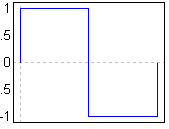
\includegraphics[scale=1.1]{haar.png}
\caption{Ondelette de Haar}
\label{haar}
\end{figure}

\subsubsection{Ondelette "chapeau mexicain" :}

On peut définir cette fonction par $\begin{array}{lrcl}
\psi : & \mathbb{R} & \longrightarrow & \mathbb{R} \\
    & t & \longmapsto & \frac{2}{\sqrt{3}}\pi^{-\frac{1}{4}}(1-t^2)e^{-\frac{t^2}{2}} \end{array}$
    
\begin{figure}[!h]
\centering
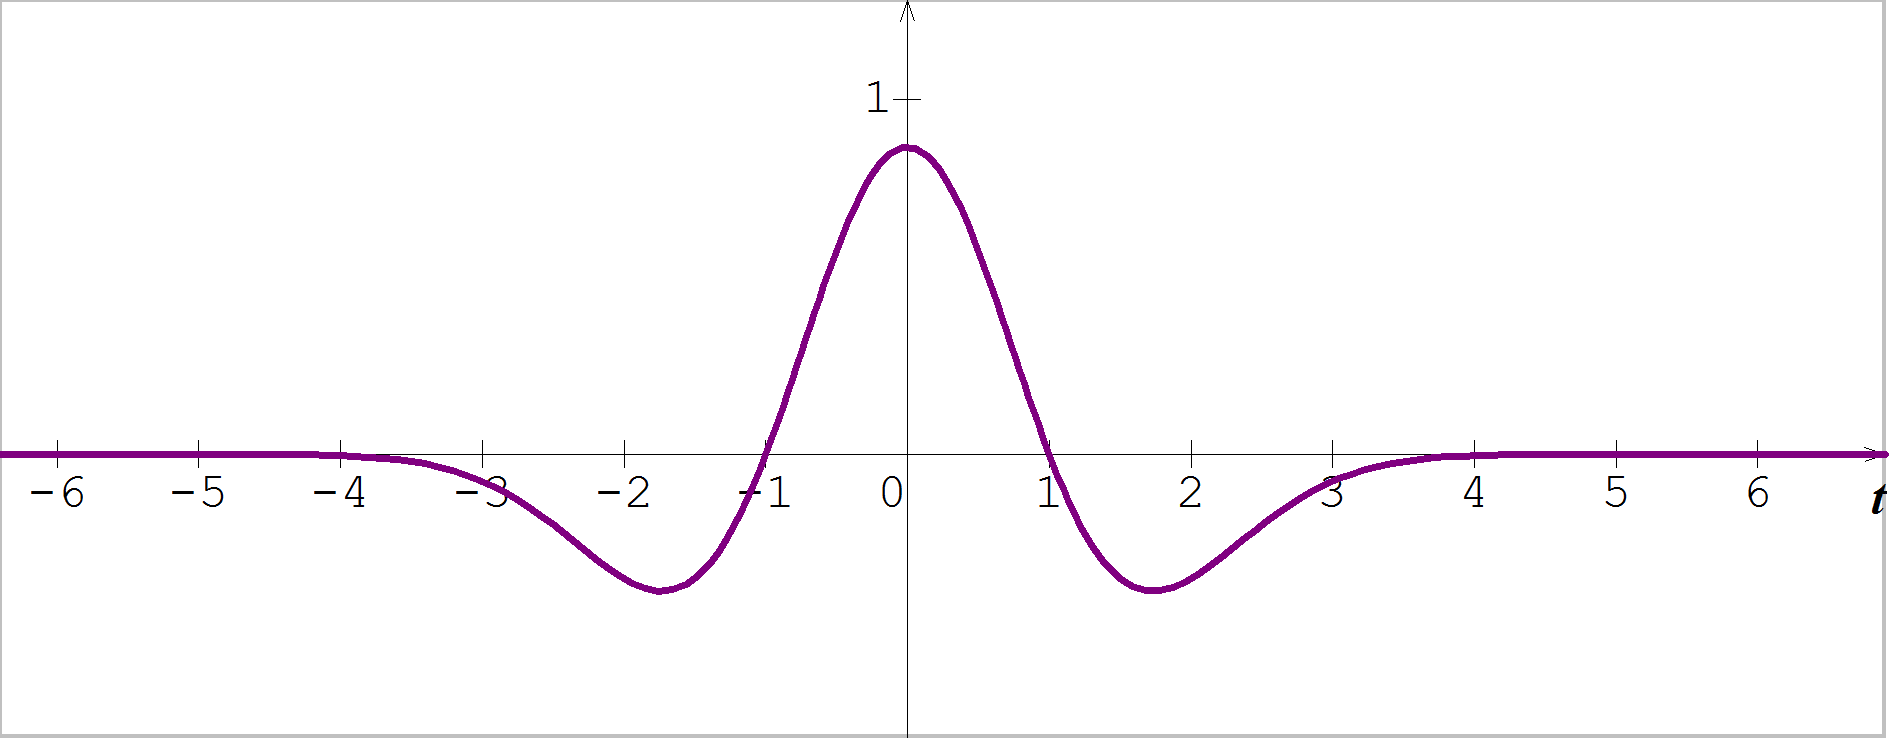
\includegraphics[scale=0.2]{chapeau_mexicain.png}
\caption{Ondelette "chapeau mexicain"}
\label{chapmex}
\end{figure}
    
\subsubsection{Ondelette de Morlet :}

On peut définir cette fonction par $\begin{array}{lrcl}
\psi : & \mathbb{R} & \longrightarrow & \mathbb{R} \\
    & t & \longmapsto & \cos(5t)e^{(-\frac{t^2}{2})} \end{array}$
    
\begin{figure}[!h]
\centering
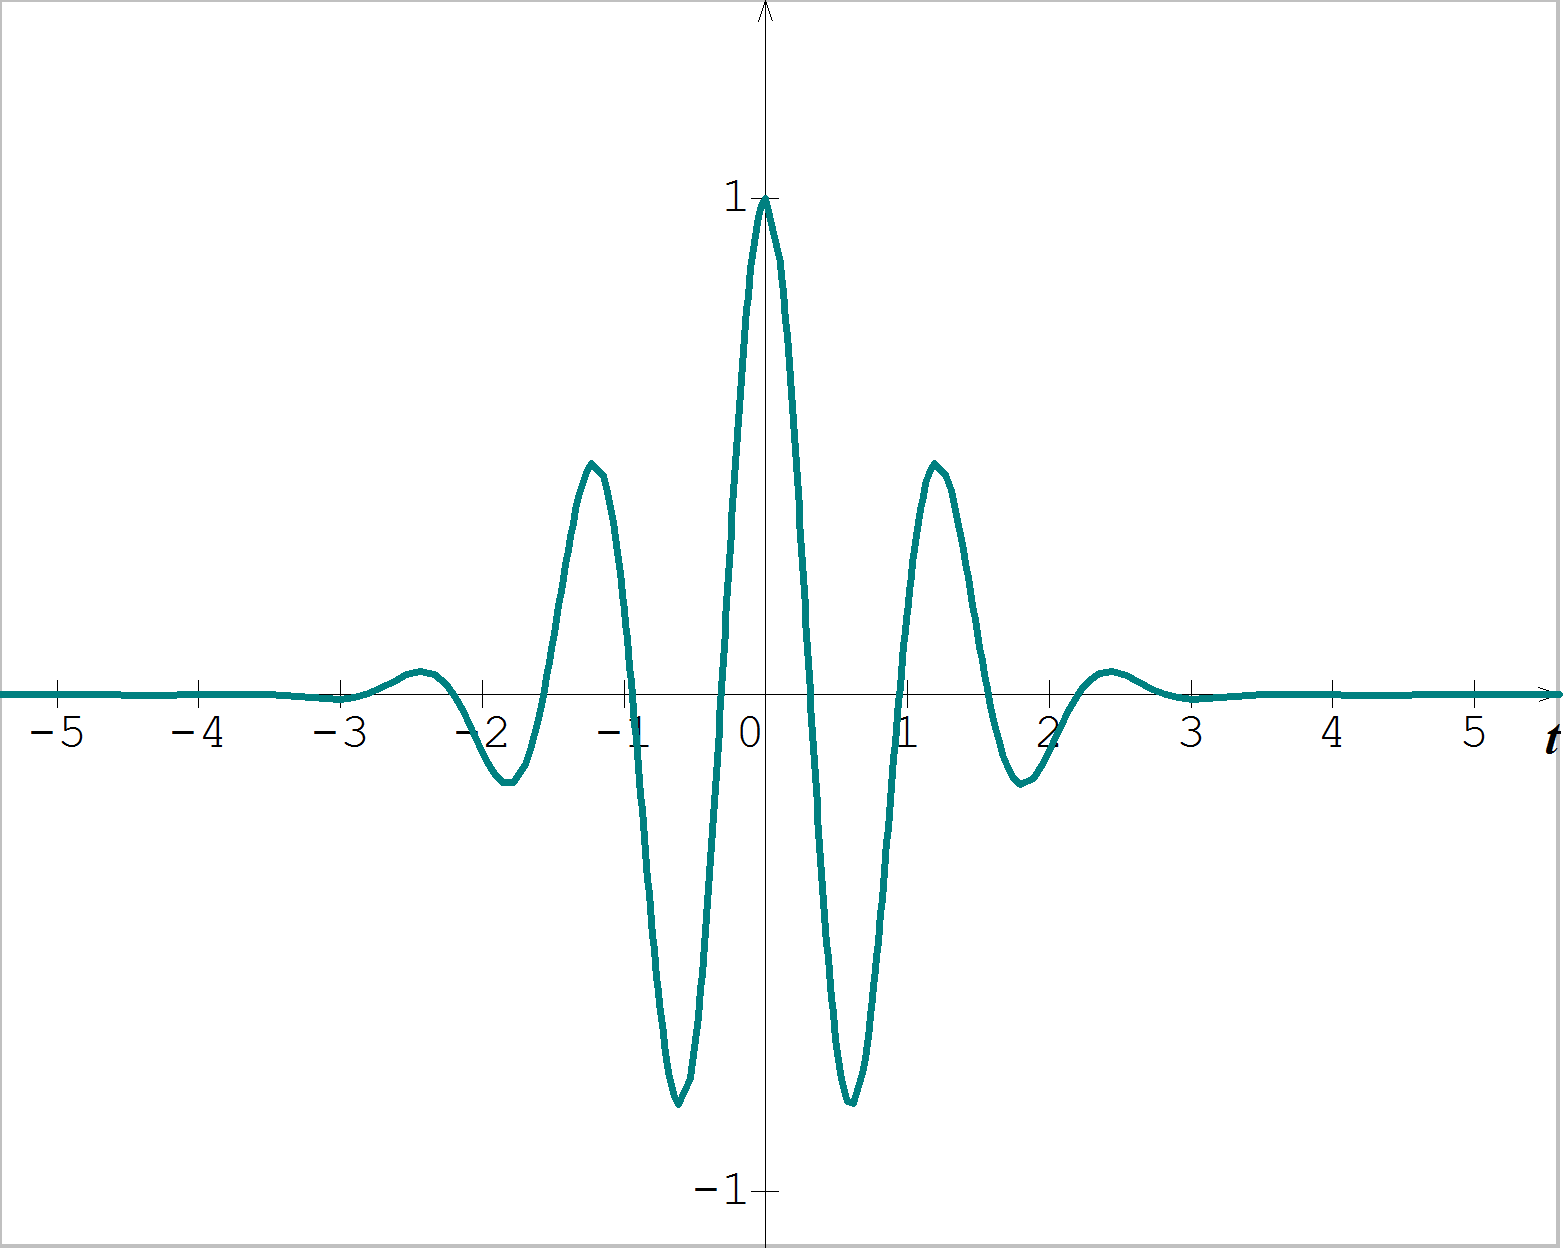
\includegraphics[scale=0.2]{morlet.png}
\caption{Ondelette de Morlet}
\label{morlet}
\end{figure}

\pagebreak

\section{Transformation en ondelettes}

La transformée en ondelettes est une transformée linéaire qui décompose un signal en fréquences en conservant une certaine localisation spatiale. Concrètement, le signal de départ est projeté sur un ensemble de fonctions de bases qui varient en fréquence et en espace. 

\subsection{Transformation en ondelette continue}

La transformée en ondelette continue utilise des dilatations et des translations de la fonction ondelette mère. 

\subsubsection*{Définition : produit scalaire}

Soient $f$ et $g$ deux fonctions réelles ; on définit sur le $\mathbb{R}$-espace vectoriel $F$($\mathbb{R}$,$\mathbb{R}$) leur produit scalaire par l’intégrale suivante : \\

$\displaystyle \langle f|g \rangle = \int_{\mathbb{R}} f(x)g(x)dx$ \\

Avec la condition d’admissibilité donnée en première page, la transformée en ondelette continue de la fonction $f$ est définie à facteur constant près comme le produit scalaire de $f$ et de $\psi$. \\

$\displaystyle \mathcal{W}_{(a,b)}(f)= \frac{1}{\sqrt{a}}\int_{-\infty}^{+\infty}f(t)\cdot\psi(\frac{t - b}{a})\cdot dt $ avec $a \in \mathbb{R}_{+}^{*}, b \in \mathbb{R}$ \\

Notons que $a$ permet de donner \textit{l’échelle} (c’est le coefficient de dilatation, de fréquence) et $b$ détermine la position de l’ondelette sur l’axe des temps.

$\frac{1}{\sqrt{a}}$ est le \textit{facteur de normalisation} de l'énergie nécessaire pour que le signal transformé ait la même énergie à toutes les échelles. \\

\textit{Ex} : \textbf{dilatation}.
L’ondelette verte a été dilatée à partir de l’ondelette rouge (ondelette-mère). On a $b = 0$ et $a \neq 1$. \\

\begin{figure}[!h]
\centering
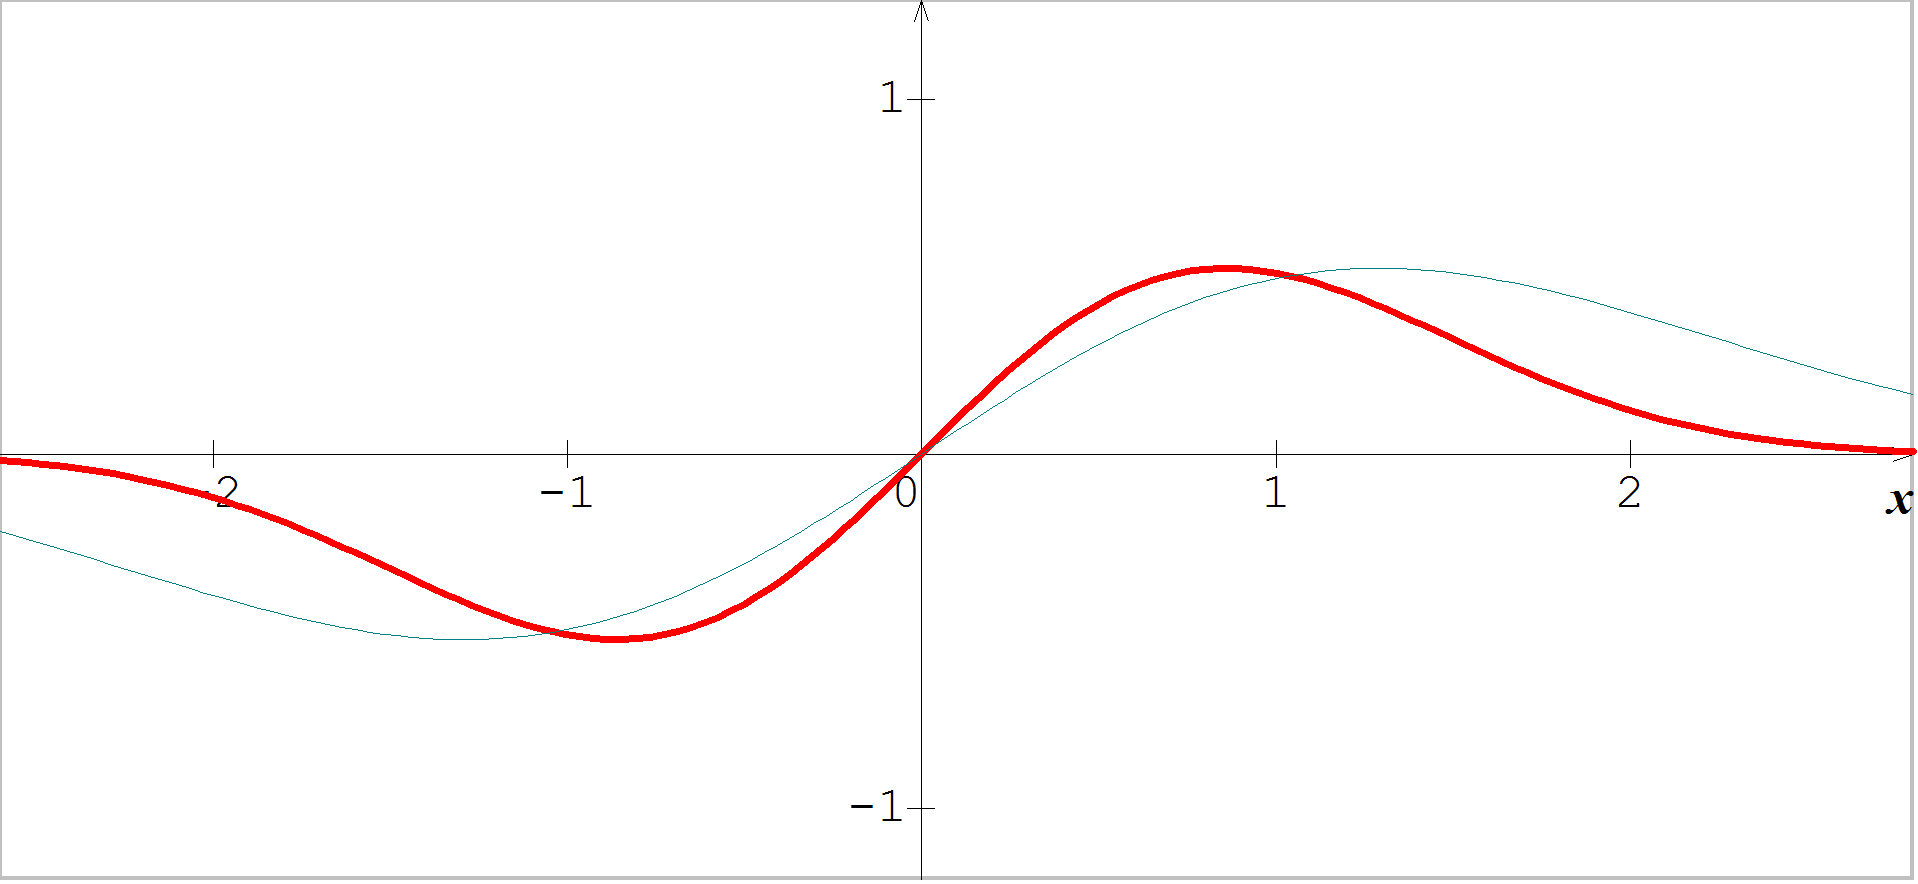
\includegraphics[scale=0.22]{dilatation.png}
\caption{Dilatation d'ondelette}
\label{dilat}
\end{figure}

\textit{Ex} : \textbf{translation}.
L’ondelette verte a été translatée à partir de l’ondelette rouge (ondelette-mère). On a $b \neq 0$ 0 et $a = 1$.

\begin{figure}[!h]
\centering
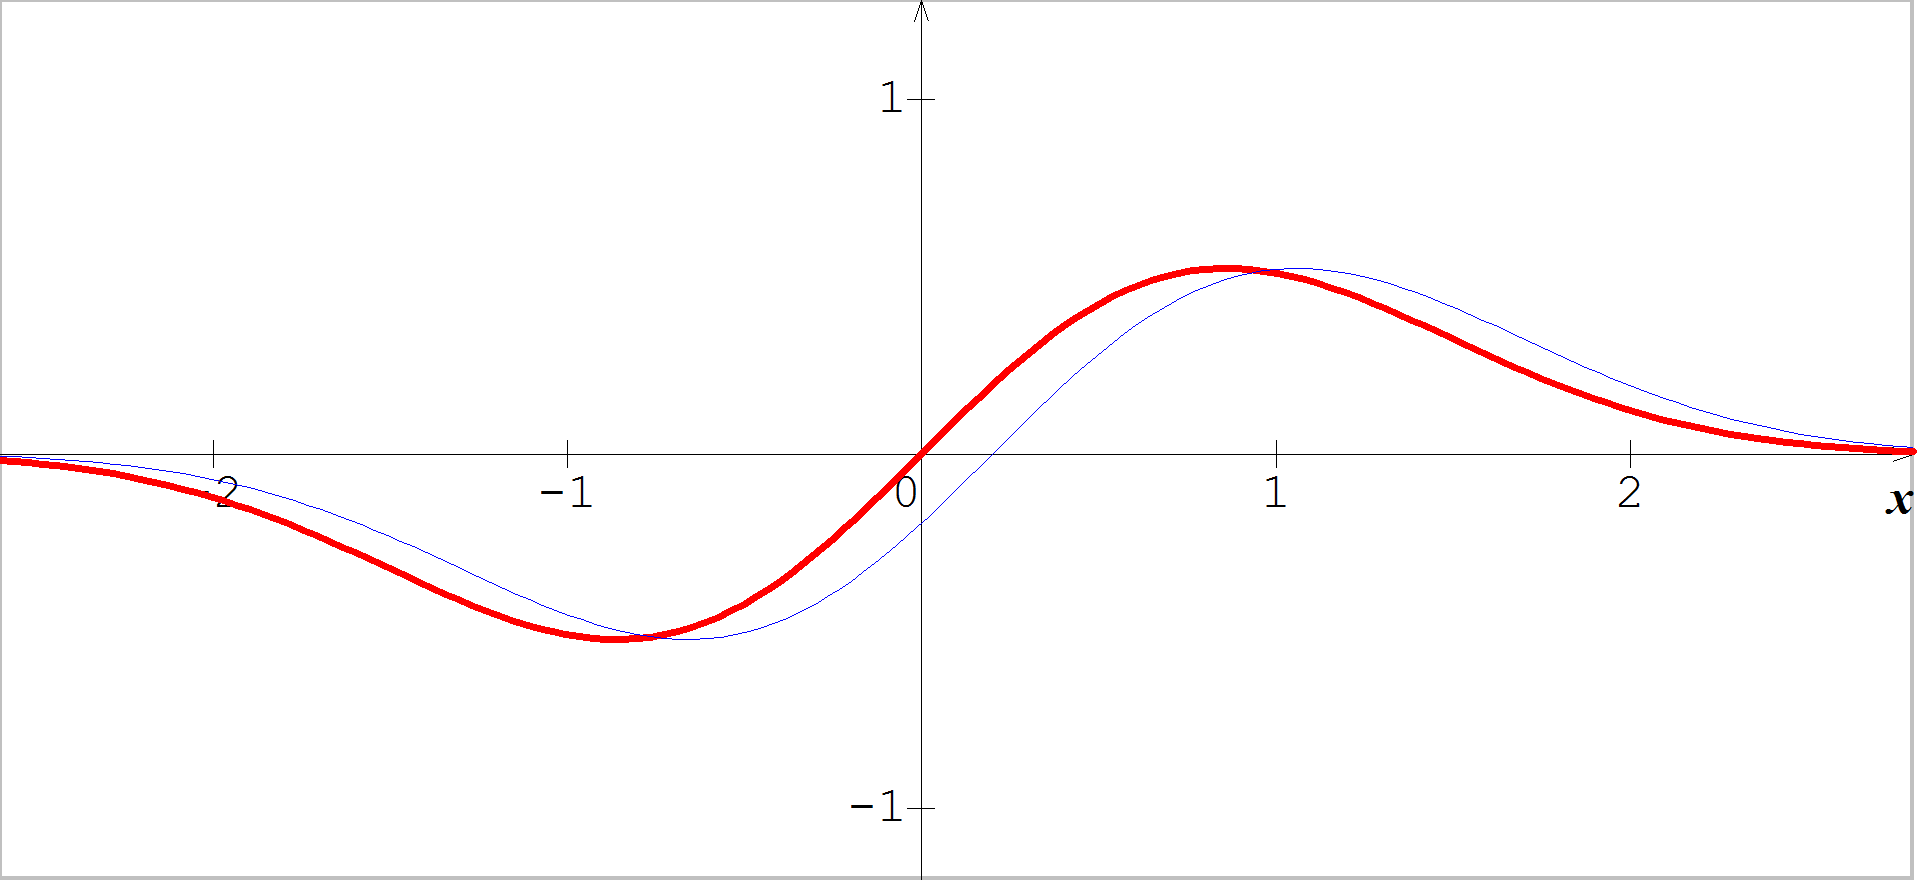
\includegraphics[scale=0.22]{translation.png}
\caption{Translation d'ondelette}
\label{translat}
\end{figure}

\subsection{Transformation en ondelettes discrète.}

La transformation en ondelettes discrète qui a été introduite par Morlet se construit à partir de << bases >> de fonctions du type : \\

$\displaystyle f_{t_{0},\Delta{}t}(t) = \frac{1}{\sqrt{\Delta{}t}}f(\frac{t-t_0}{\Delta{}t}) \text{ avec } \Delta{}t > 0, t_0 \in \mathbb{R}$ \\

$\Delta{}t$ peut être choisi << géométriquement >>; les paramètres de translations $t_0$ et $\Delta{}t$ son proportionnels (c'est-à-dire $\exists k \in \mathbb{R}, t_0 = k\cdot{}\Delta{}t$).

Une gamme d'échelles $\Delta{}t$ utilisée couramment est la gamme d'échelles dyadiques $\frac{1}{2^p}$

On a alors avec $t_0 = k\cdot\Delta{}t$ : \\

$\displaystyle f_{t_{0},\Delta{}t}(t) = 2^{\frac{p}{2}}f(2^{p}\cdot{}x - k)$, c'est-à-dire on peut considérer la famille d'ondelettes $\psi{}_{k,p} = 2^{\frac{p}{2}}\psi{}(2^{p}x - k ), (k,p) \in \mathbb{Z}^2$ \\

Il est intéressant de considérer des familles orthogonales d'ondelettes formant une base hilbertienne de $L^2(\mathbb{R})$ alors toute fonction $f$ de cet espace peut s'écrire 

$\displaystyle f = \sum_{(k,p) \in \mathbb{Z}^2}f_{k,p}\psi{}_{k,p}$ où les $f_{k,p} = \langle{}f|\psi_{k,p}\rangle$ sont appelés coefficients d'ondelettes.

La transformation en ondelettes discrète est presque naturellement associée à des algorithmes plus efficaces et plus rapides que des algorithmes du type FFT qui utilisent la transformée de Fourier.

Une famille d’ondelettes par exemple couramment utilisée dans la transformation en ondelettes discrète est la famille infinie des ondelettes orthogonales de Daubechies : c’est une des familles d’ondelettes les plus performantes.


\section{la théorie de l'analyse multirésolution, outil pour la construction de bases d'ondelettes}

Pour construire des bases d'ondelettes orthonormées, les théoriciens Mallat et Meyer ont introduit la notion d'analyse multirésolution.

\subsection{Définition d'une analyse multirésolution.}

Une analyse multirésolution est une suite $\{V_k\}_{k\in\mathbb{Z}}$ de sous-espaces fermés de $\mathcal{L}^2(\mathbb{R})$ tels que : \\

\begin{itemize}
\item $\forall{}(k,l) \in \mathbb{Z}^2, f \in V_k \leftrightarrow f(\cdot - 2^{k}l) \in V_k $ (propriété d'invariance par translation)

\item $\forall k \in \mathbb{Z}, V_{k+1} \subset V_k$

\item $\forall k \in \mathbb{Z}, f \in V_k \leftrightarrow f(\frac{\cdot}{2}) \in V_{k+1}$

\item $\displaystyle \lim_{j \to \infty} V_k = \bigcap{}_{k\in\mathbb{Z}}V_k = \emptyset $

\item $\displaystyle \lim_{j \to -\infty} V_k = \overline{\bigcap{}_{k\in\mathbb{Z}}V_k} = \mathcal{L}^2(\mathbb{R}) $ où la notation $\bar{A}$ désigne l'adhérence de $A$.

\item $\exists\phi, \{\phi(\cdot - n)\}_{n \in \mathbb{Z}}$ forme une base orthonormée de $V_0$. $\phi$ est appelée fonction d'échelle associée à l'analyse multirésolution
\end{itemize}

\subsection{Intéret d'une analyse multirésolution}

La fonction $\phi$ permet notamment la connaissance de la suite $\{V_k\}_{k\in\mathbb{Z}}$ et ainsi la déduction d'une base orthonormée de $V_k$ pour tout $k \in \mathbb{Z}$. On peut alors définir une ondelette associée à l'analyse multirésolution : il s'agira de toute fonction $\psi$ qui forme avec ses translatées entières une base orthonormée de $W_0$, supplémentaire orthogonal de $V_1$ dans $V_0$. En effet, il découle de la définition de $W_k$ que $\displaystyle \mathcal{L}^2(\mathbb{R}) = \overline{\bigoplus{}_{k\in\mathbb{Z}}W_k}$. \\

Par suite, la famille $\displaystyle \{\frac{1}{\sqrt{2^m}}\psi(\frac{\cdot - 2^{m}n}{2^m})\}_{(m,n)\in\mathbb{Z}^2}$ forme une base orthonormée de $\mathcal{L}^2(\mathbb{R})$.

Les espaces $W_k$ pour $k\in\mathbb{Z}$ sont appelés espaces des détails. Ils ne forment pas une famille d'espaces emboîtés mais les propriétés d'échelles et d'invariance par translation sont conservées. En effet, pour $k \in \mathbb{Z}, X_{k-1}$ est orthogonal à $V_{k-1}$, d'où $W_{k-1}$ orthogonal à $W_k$ en vertu de l'égalité $\displaystyle \mathcal{L}^2(\mathbb{R}) = \overline{\bigoplus{}_{k\in\mathbb{Z}}W_k}$.




\section{Algorithme de decomposition en ondelettes de Stephane Mallat (1989)}

\subsection{Principe}

C’est un algorithme linéaire qui fait appel à un sous-échantillonnage. Concrètement, on procède à une décomposition par projections successives (c’est-à-dire de manière récursive) sur deux sous-espaces orthogonaux, l’un donnant l’allure générale de l’image (il s'agira de l'image en résolution moitié) et l’autre les détails. 
L’algorithme de Mallat a cependant le défaut de ne pas être invariant par translation.

On peut donner une démonstration mathématique de cet algorithme ; ici, pour simplifier, on va se limiter au cas particulier de décomposition d’un signal par les ondelettes de Haar.


\subsection{Démonstration dans un cas simple : le cas des ondelettes de Haar.}

La démonstration suivante montre comment on calcule les coefficients des ondelettes de Haar : on est bien évidemment dans le cadre d'une transformation en ondelettes discrètes.

\subsubsection{Introduction et définition des notations}

Considérons un signal échantillonné régulièrement sur [0,1] en $2^p$ points notés $x_{k}$ avec $x_{k} = \frac{k}{2^p}$.

On associe à cet échantillon une fonction $f$ définie par $f(x) = \begin{cases}
     f_{k} \text{ si } x \in I_{k} = [x_{k},x_{k+1}[\\
     0 \text{ sinon }
   \end{cases}$.
Quand l'échantillonnage varie, $f$ varie en décrivant l'ensemble $\mathbb{K}_{p}$ des fonctions constantes sur chacun des intervalles $I_{k}$ et nulles sur $\mathbb{K} \setminus [0,1]$. \\

$F$($\mathbb{R}$,$\mathbb{R}$), ensemble des fonctions réelles à valeurs réelles, est un $\mathbb{R}$-espace vectoriel et on montre facilement que $\mathbb{K}_{p}$ est un sous-espace vectoriel de $F$($\mathbb{R}$,$\mathbb{R}$. \\

De plus, pour $p \in \mathbb{N}$, on a $\mathbb{K}_{0} \subset \mathbb{K}_{1} \subset .. \subset \mathbb{K}_{p} \subset \mathbb{K}_{p+1} \subset ... $ ce qui montre $\bigcup\limits_{p \in \mathbb{N}}\mathbb{K}_{p}$ est un sous-espace vectoriel de $F$($\mathbb{R}$,$\mathbb{R}$).

\uppercase{à} partir de la fonction de Haar $H$, on définit la fonction $H_{p,k}$ par $H_{p,k}(x) = H(2^{p}x - k). (p,k) \in \mathbb{N}^2$.

\textit{[Pour alléger l’écriture et les calculs, on peut comme ici choisir d’omettre le facteur }$2^\frac{p}{2}$ devant $ H(2^{p}x - k)$.] \\

Soit la fonction définie par \[
 h_{p,k}(x) = \begin{dcases*}
        1 \text{ si } x \in I_{k} = [ \frac{k}{2^p},\frac{k+1}{2^p}[ \\ 
        0 \text{ sinon }
        \end{dcases*}
 = h(2^{p}x - k) \] (avec $h$ définie comme la fonction de Haar mais associant 1 quel que soit $x \in [0,1]$.). \\

Or toute fonction $f$ de $\mathbb{K}_{p}$ se décompose de manière unique sous la forme : \\

$\displaystyle f = \sum_{k = 0}^{2^p - 1} f_{k}h_{p,k} = f_{0}h_{p,0} + f_{1}h_{p,1} + ... + f_{2^p - 1}h_{p,2^p - 1}$ \\

On a bien $\forall x \in [0,1[, f(x) = f_0 \times \begin{cases} 1 \text{ si } x \in I_0 \\ 0 \text{ sinon } \end{cases}
+ f_1 \times \begin{cases} 1 \text{ si } x \in I_1 \\ 0 \text{ sinon } \end{cases}
+ ... +
f_{2^p - 1} \times \begin{cases} 1 \text{ si } x \in I_{2^p - 1} \\ 0 \text{ sinon } \end{cases} $.\\

D'où $(h_{p,0},h_{p,1},...,h_{p,2^p -1})$ est une base de $\mathbb{K}_p$.\\



Avec $F(\mathbb{R},\mathbb{R})$ muni du produit scalaire défini en \textit{définition 2}, on a : \\

\begin{itemize}

\item Si $k \neq k'$ :

$\displaystyle \langle h_{p,k}|h_{p,k'} \rangle = \int_{0}^{1} h_{p,k}(x)\cdot{}h_{p,k'}(x) = \int_0^1 0\cdot{}dx = 0$ \\

\item Si $k = k'$ :

\begin{align*} \displaystyle
\langle h_{p,k}|h_{p,k'} \rangle &= \int_{0}^{1} (h_{p,k}(x))^2 dx \\
 &= \int_{0}^{x_k} h_{p,k}(x))^2 dx + \int_{x_k}^{x_{k+1}} h_{p,k}(x))^2 dx + \int_{x_{k+1}}^{1} h_{p,k}(x))^2 dx  \\
\displaystyle &= \int_0^{x_k} 0^2 dx + \int_{x_k}^{x_{k+1}} 1^2 dx + \int_{x_{k+1}}^{1} 0^2 dx = 0 + [x]_{x_k}^{x_{k+1}} + 0 = x_{k+1} - x_k  \\
\displaystyle &= \frac{1}{2^p} \\
\end{align*} 
\end{itemize}

Ainsi la base $(h_{p,0},h_{p,1},...,h_{p,2^p -1})$ est une base orthogonale ; ce qui fait des espaces $\mathbb{K}_p$ des espaces euclidiens.


\subsubsection{Propriété mathématique : Orthogonalité dans les espaces euclidiens}
\paragraph{\uppercase{é}noncé}
Soient $E$ un espace euclidien de dimension $n \geq 1$, $\langle .| .\rangle$ son produit scalaire et $F$ un sous-espace vectoriel de $E$.

Alors $F$ admet un supplémentaire orthogonal dans $E$ et ce supplémentaire est unique. On le note : $F^{\perp}$.
 \\
 \\
\paragraph{Démonstration} :

\begin{itemize}

\item Existence :

\begin{itemize}


\item Si $F = \{0_E\}$, on a $E = F \oplus E$ de manière immédiate. De plus, si $y \in F, y = 0_E$ et $\forall x \in E, \langle x|0_E \rangle = 0 $. D'où E est un supplémentaire orthogonal à $F$. \\

\item Si $F = E$, par un raisonnement analogue, on trouve que $\{0_E\}$ est un supplémentaire orthogonal à $F$. \\

\item Si $F \neq \{0_E\}$ et $F \neq E$, on considère $(e_i)_{1\leq{}i\leq{}p}$ une base orthonormale de $F$ avec $p =$ dim $F \in \mathbb{N}^{*}.$ \\

L'ensemble $F^{\perp} = \{ x \in E | \forall y \in F, \langle x|y \rangle = 0 \}$ est par définition orthogonal à $F$. \\

Soit $x \in E$.

$\exists (\lambda{}_{1}, ..., \lambda{}_{p}) \in \mathbb{R}^p , x = \sum_{k = 1}^{p} \lambda{}_{k}e_k + (x - \sum_{k = 1}^{p} \lambda{}_{k}e_k)$

Or le premier vecteur de la somme est dans $F$. Donc le second entre parenthèses appartient à $F^{\perp}$ si et seulement si 

$\displaystyle \forall k \in [|1,p|], \langle e_k | x - \sum_{k = 1}^{p}\lambda{}_{k}e_k \rangle = 0$, c'est-à-dire $\lambda_{k} = \langle e_k | x \rangle$

Avec $x$ écrit de la manière suivante, on établit ainsi que  $E = F + F^{\perp}$.

$\displaystyle x = \sum_{k = 1}^p \langle e_k | x \rangle{}\cdot{}e_k + (x - \sum_{k = 1}^p \langle e_k | x \rangle{}\cdot{})$

On a aussi immédiatement $F \cap F^{\perp} = \{0_E\}$, ce qui établit $E = F \oplus F^{\perp}$ et ainsi l'existence d'un supplémentaire orthogonal à $F$ 
\end{itemize}

\item Unicité :

Soit $G$ un sous-espace vectoriel supplémentaire de $F$ dans $E$ et orthogonal à $F$.

On a déjà $G \subset F^{\perp}$ puisque tous les vecteurs de G sont orthogonaux à tous les vecteurs de $F$.

De plus, dim $G$ = dim $E -$ dim $F$ = dim $F^{\perp}$ car $\begin{dcases} E = F \oplus F^{\perp} \\ E = F \oplus G \end{dcases}$; on en déduit $G = F^{\perp}$ et l'unicité du supplémentaire orthogonal. \\
\end{itemize}

\subsubsection{Utilisation de la propriété : décomposition orthogonale en somme directe.}

Soit donc $\mathbb{S}_{p}$ le supplémentaire orthogonal de $\mathbb{K}_p$ dans $\mathbb{K}_{p+1}$. \\

On a $\mathbb{K}_{p+1} = \mathbb{S}_{p} \oplus \mathbb{K}_p$. D'où de proche en proche on arrive à :

$\mathbb{K}_{p+1} = \mathbb{S}_{p} \oplus \mathbb{S}_{p-1} \oplus \mathbb{S}_{p-2} \oplus ... \oplus \mathbb{S}_{0} \oplus \mathbb{K}_{0}$, soit encore $\mathbb{K}_p = \mathbb{K}_0 \oplus{}_{i = 0}^{p-1} \mathbb{S}_{i	} $ \\

On a défini à partir de $\mathcal{H}$ la fonction $H_{p,k}$ par $H_{p,k}(x) = \mathcal{H}(2^{p}x - k )$; $(p,k) \in \mathbb{N}^2$.

On alors $H_{p,k}(x) =  \begin{dcases} 1 \text{ si } x \in [\frac{k}{2^p};\frac{k + \frac{1}{2}}{2^p}[ \\ 
-1 \text{ si } x \in [\frac{k + \frac{1}{2}}{2^p};\frac{k + 1}{2^p}[ \\
0 \text{ dans les autres cas } \end{dcases}$.

Facilement, on montre que $(h_{p,1},h_{p,0},...,h_{p,2^p - 1},H_{p,0},H_{p,1},...,H_{p,2^p - 1})$ forme une base de $\mathbb{K}_{p+1}$.

De plus, on a :

\begin{itemize}

\item Si $k \neq k'$

\begin{align*}
\langle h_{p,k}|H_{p,k'} \rangle &= \int_{0}^1 h_{p,k}(x)\cdot{}H_{p,k'}(x)\cdot{dx} \\ 
&= \int_{0}^{x_k} 0 dx + \int_{x_k}^{x_{k+1}} 1\cdot{}0dx + \int_{x_{k+1}}^{x_{k'}} 0dx + \\
 &\int_{x_{k'}}^{\frac{x_{k'} + x_{k'+1} }{2}} 0\cdot{}1dx + \int_{\frac{x_{k'} + x_{k'+1} }{2}}^{x_{k'+1}} 0(-1)dx + \int_{x_{k'+1}}^{1} 0.dx \\
&= 0
\end{align*} 
\item Si $k =k'$

\begin{align*}
 \langle h_{p,k}|H_{p,k'} \rangle &= \int_{0}^1 h_{p,k}(x)\cdot{}H_{p,k'}(x)\cdot{dx} \\
&= \int_{0}^{x_k} 0dx + \int_{x_k}^{x_{k+1}} 1\cdot{}H_{p,k}(x)dx + \int_{x_{k+1}^1} 0\cdot{}dx \\
&= \int_{x_{k'}}^{\frac{x_{k'} + x_{k'+1} }{2}} 1dx + \int_{\frac{x_{k'} + x_{k'+1} }{2}}^{x_{k'+1}} -1dx \\
&= 0 . \\
\end{align*}
\end{itemize}

De ce qui précède, il résulte que $(h_{p,1},h_{p,0},...,h_{p,2^p - 1},H_{p,0},H_{p,1},...,H_{p,2^p - 1})$ forme une base orthogonale de $\mathbb{K}_{p+1}$.

Alors le système $(H_{p,0}, H_{p,1},..., H_{p,2^p - 1},)$ est une base orthogonale de l'orthogonal $\mathbb{S}_{p}$ de $\mathbb{K}_{p}$ dans $\mathbb{K}_{p+1}$.

De plus, on peut déjà remarquer :

$\displaystyle \langle H_{p,k}|H_{p,k} \rangle = \int_0^1 (H_{p,k}(x))^{2}\cdot{}dx = \int_{x_{k'}}^{\frac{x_{k'} + x_{k'+1} }{2}} 1^{2}\cdot{}dx + \int_{\frac{x_{k'} + x_{k'+1} }{2}}^{x_{k'+1}} (-1)^{2}\cdot{}dx = \frac{1}{2^p} $ \\


-Soit un signal $\Psi{}_{p} \in \mathbb{K}_{p}$. \\ Alors $\displaystyle \exists{}! (\Psi{}_{p,0},\Psi{}_{p,1},...,\Psi{}_{p,2^p - 1},) \in \mathbb{R}^{2^p}, \Psi{}_{p} = \sum_{k=0}^{2^p - 1} \Psi{}_{p,k}h_{p,k}$.

Puisque $\mathbb{K}_{p} = \mathbb{K}_{p-1} \oplus \mathbb{S}_{p-1}, \exists{}!(\Psi{}_{p-1},d_{p-1}) \in \mathbb{K}_{p-1} \times \mathbb{S}_{p-1}, \Psi{}_p = \Psi{}_{p-1} + d_{p-1} $. \\

Et on peut décomposer $\Psi{}_{p-1}$ et $d_{p-1}$ comme suit :

$\displaystyle \Psi{}_{p-1} = \sum_{k=0}^{2^p - 1} \Psi{}_{p-1,k}h_{p-1,k}$ et $d_{p-1} = \sum_{k=0}^{2^p - 1} d_{p-1,k}H_{p-1,k}$. \\

\subsubsection{\uppercase{é}tape principale de l'algorithme : passage à la résolution inférieure, détermination des coefficients à la résolution inférieure.}

-Déterminons les $\Psi{}_{p-1,k}$ et $d_{p-1,k}$ :

\paragraph{Premières égalités}
L'orthogonalité de la base $(h_{p,1},h_{p,0},...,h_{p,2^p - 1},H_{p,0},H_{p,1},...,H_{p,2^p - 1})$ avec $\Psi{}_{p} = \Psi{}_{p-1} + d_{p-1}$ et les résultats précédents sur les produits scalaires amène à : $\langle \Psi{}_{p}|h_{p-1,k} \rangle = \frac{\Psi{}_{p-1,k}}{2^{p-1}}$ et $\langle \Psi{}_{p}|H_{p-1,k} \rangle = \frac{d_{p-1,k}}{2^{p-1}}$. \\

\subparagraph*{Démonstration} 

On a \begin{align*}
 \langle\Psi{}_{p}|h_{p-1,k} \rangle &= \langle \Psi{}_{p-1}|h_{p-1}\rangle + \langle d_{p-1}|h_{p-1,k} \rangle  \text{ par linéarité du produit scalaire.} \\
 &= \sum_{i \neq k} \Psi{}_{p-1,i} \langle h_{p-1,i}|h_{p-1,k} \rangle + \Psi{}_{p-1,k} \langle h_{p-1,k}|h_{p-1,k} \rangle + \sum_{i=0}^{2^{p-1} - 1} d_{p-1,i}\langle H_{p-1,i}|h_{p-1,k} \rangle  \\
 &= \sum_{i \neq k} \Psi{}_{p-1,i}\cdot{}0 + \frac{\Psi{}_{p-1,k}}{2^{p-1}} + \sum_{i=0}^{2^{p-1} - 1} d_{p-1,i}\cdot{}0 = \frac{\Psi{}_{p-1,k}}{2^{p-1}} 
 \end{align*}

Et on a 
\begin{align*} \displaystyle
 \langle\Psi{}_{p}|H_{p-1,k} \rangle &= \langle \Psi{}_{p-1}|H_{p-1}\rangle + \langle d_{p-1}|h_{p-1,k} \rangle  \\
&= \sum_{i=0}^{2^{p-1}-1} \Psi{}_{p-1,i}\langle h_{p-1,i}|H_{p-1,k}\rangle + \sum_{i \neq k}d_{p-1,i}\langle{}H_{p-1,i}|H_{p-1,k} \rangle + d_{p-1,k}\langle{}H_{p-1,k}|H_{p-1,k}\rangle  \\
&= \sum_{i=0}^{2^{p-1}-1}\Psi{}_{p-1,i}\cdot{}0 + \sum_{i \neq k}d_{p-1,i}\cdot{}0 + d_{p-1,k}\langle{}H_{p-1,k}|H_{p-1,k} \\ &= \frac{d_{p-1,k}}{2^{p-1}}
\end{align*} \\

\paragraph{Secondes égalités}

D'autre part, on peut montrer $\displaystyle \langle{}\Psi{}_{p}|h_{p-1,k}\rangle = \frac{\Psi{}_{p,2k} + \Psi{}_{p,2k + 1} }{2^p}$ et $\displaystyle \langle{}\Psi{}_{p}|H_{p-1,k}\rangle = \frac{\Psi{}_{p,2k} - \Psi{}_{p,2k + 1} }{2^p}$ \\


\subparagraph*{Démonstration} 

On a $\displaystyle \langle{}h_{p,k}|h_{p-1,k'}\rangle = \int_0^1 h_{p,k}(x)\cdot{}h_{p-1,k'}(x)\cdot{}dx = \int_{x_k}^{x_{k+1}}h_{p-1,k'}(x)\cdot{}dx$ \\

Or, on sait par définition que \[ h_{p-1,k'}(x)= \begin{dcases} 1 \text{ si }x \in [\frac{k'}{2^{p-1}};\frac{k'+1}{2^{p-1}}] \\
0 \text{ sinon } \end{dcases} \]\\
D'où :
\[ \begin{dcases}
\langle{}h_{p,k}|h_{p-1,k'}\rangle = \int_{x_k}^{x_{k+1}}1\cdot{}dx
= \frac{1}{2^p} \text{ si } \frac{k'}{2^{p-1}} \leq x_k \leq x_{k+1} \leq \frac{k'+1}{2^{p-1}}, \text{ ou encore } k \in \{2k',2k'+1\}\\ 
\langle{}h_{p,k}|h_{p-1,k'}\rangle = \int_{x_k}^{x_{k+1}0\cdot{}dx = 0 si k \notin \{2k',2k'+1\}}
\end{dcases} \]

On a de même \\
 $\displaystyle \langle{}h_{p,k}|H_{p-1,k'}\rangle = \int_0^{1}h_{p,k}(x)\cdot{}H_{p-1,k'}(x)\cdot{}dx = \int_{x_k}^{}x_{k+1}H_{p-1,k'}(x)\cdot{}dx$

On sait par définition que \[ H_{p-1,k'}(x) = \begin{dcases} 
1 \text{ si } x \in [\frac{k'}{2^{p-1}};\frac{k'+\frac{1}{2}}{2^{p-1}}] \\
-1 \text{ si } x \in [\frac{k'+\frac{1}{2}}{2^{p-1}};\frac{k'+1}{2^{p-1}} \\
0 \text{ sinon }
\end{dcases}
\] D'où :

\[ \begin{dcases}
\langle{}h_{p,k}|H_{p-1,k'}\rangle = \int_{x_k}^{x_{k+1}}1\cdot{}dx = \frac{1}{2^p} \text{ si } \frac{k'}{2^{p-1}} \leq x_k \leq x_{k+1} \leq \frac{k'+\frac{1}{2}}{2^{p-1}}, \text{ ou encore } k = 2k' \\
\langle{}h_{p,k}|H_{p-1,k'}\rangle = \int_{x_k}^{x_{k+1}}-1\cdot{}dx = -\frac{1}{2^p} \text{ si } \frac{k'+\frac{1}{2}}{2^{p-1}} \leq x_k \leq x_{k+1} \leq \frac{k'+1}{2^{p-1}}, \text{ soit } k = 2k'+1 \\
\langle{}h_{p,k}|H_{p-1,k'}\rangle = \int_{x_k}^{x_{k+1}}0\cdot{}dx = 0 si k \notin \{2k',2k'+1\}
\end{dcases}
\]

\uppercase{à} partir de cela, il est facile de décomposer comme suit et d'obtenir les résultats :

\begin{itemize}
\item \begin{align*}\displaystyle \langle \Psi{}_{p}|h_{p-1,k}\rangle &=  \langle \sum_{k=0}^{2^{p-1}}\Psi{}_{p,k}h_{p,k}|h_{p-1,k}\rangle \\ &=  \sum_{i\notin{}\{2k',2k'+1\}}\Psi{}_{p,i}\langle{}h_{p,i}|h_{p-1,k}\rangle + \sum_{i\notin{}\{2k',2k'+1\}}\Psi{}_{p,i}\langle{}h_{p,i}|h_{p-1,k}\rangle  \\ 
&= 0 + \Psi{}_{p,2k}\cdot{}\frac{1}{2^p} + \Psi{}_{p,2k+1}\cdot{}\frac{1}{2^p} 
\end{align*} 

\item \begin{align*} \displaystyle \langle \Psi{}_{p}|H_{p-1,k}\rangle &= \langle \sum_{k=0}^{2^{p-1}}\Psi{}_{p,k}h_{p,k}|H_{p-1,k}\rangle \\ &= 
 \sum_{i\notin{}\{2k',2k'+1\}}\Psi{}_{p,i}\langle{}h_{p,i}|H_{p-1,k}\rangle + \sum_{i\notin{}\{2k',2k'+1\}}\Psi{}_{p,i}\langle{}h_{p,i}|h_{p-1,k}\rangle  \\ 
&= 0 + \Psi{}_{p,2k}\cdot{}\frac{1}{2^p} + \Psi{}_{p,2k+1}\cdot{}\frac{-1}{2^p}
\end{align*} \\


\end{itemize}

\paragraph{Conclusion}

On obtient finalement avec les égalités encadrées les équations d'échelles suivantes. \\

\[ \begin{dcases} \Psi{}_{p-1,k} = \frac{\Psi{}_{p,2k} + \Psi{}_{p,2k}}{2}  \| (\Psi{}_{p-1,k})_{k\in{}[|0;2^{p-1}-1|]} \text{est la famille des coefficients d'approximation à la résolution} 2^{p-1} \\ 
d_{p-1,k} = \frac{\Psi{}_{p,2k} - \Psi{}_{p,2k}}{2}  \| (d_{p-1,k})_{k\in{}[|0;2^{p-1}-1|]} \text{est la famille des coefficients d'ondelettes}
\end{dcases} \] 

Ainsi, lorsqu’on connaît les coefficients d’ondelettes à un niveau de résolution $p$, on peut aisément déterminer ceux du niveau $p-1$ et l’égalité des sous-espaces vectoriels en somme directe se comprend par :

$$ \underbrace{\mathbb{K}_p}_{\text{Signal à la résolution } 2^p}
= \underbrace{\mathbb{K}_{p-1}}_{\text{Signal à la résolution } 2^{p-1}} \oplus 
\underbrace{\mathbb{S}_{p-1}}_\text{Détails (ou pertes)} $$

L’intérêt principal de cet algorithme est qu’il permet de passer d’un échantillon de taille $2^p$ à un nouvel échantillon principal de taille $2^{p-1}$ et un échantillon de taille $2^{p-1}$ en utilisant que des sommes ou des différences.


\subsection{Shématisation de l'algorithme de Mallat (compression d'un signal $\Psi{}_{p}$ par des ondelettes)} 

\begin{tabular}{cccc}
           &             & Etape 1      & \\
$\Psi{}_{p}$ & $\rightarrow$ & $\Psi{}_{p-1}$ & \\
           & $\searrow$    & $d_{p-1}$      & (détails)
\end{tabular} \\

En réitérant le processus jusqu’à la dernière étape (étape $p$), on obtient la configuration suivante : \\


\begin{tabular}{ccccccccc}
           &             & Etape 1      & 			  & Etape 2     & & & & Etape p \\
$ \Psi{}_{p}$ & $ \rightarrow$ & $ \Psi{}_{p-1}$ & $ \rightarrow$ & $ \Psi{}_{p-2}$ & $ \rightarrow$ & ... & $ \rightarrow$ & $ \Psi{}_0$ \\
           & $ \searrow$    & $ d_{p-1} $      & $ \searrow$    & $ d_{p-2} $ 
& $ \searrow $ & $ d_{p-3 }$ & $ \searrow $ & $ d_0 $
\end{tabular} \\

Ce travail est en réalité la première partie de l’algorithme, appelée \textit{analyse}. \\

Il s’ensuit une deuxième partie appelée \textit{synthèse}, qui correspond à l’opération inverse de l’analyse. Dans cette partie, les coefficients d’ondelettes << omis >> dans l’analyse entraînent des erreurs.

Notons toutefois que l’algorithme posé par Stéphane Mallat se fonde sur la notion d’analyse multirésolution de $L^2 (\mathbb{R})$ (qui a été d’ailleurs introduite afin de construire des bases orthogonales d’ondelettes). Il s’agit toutefois comme ici d’une suite de sous-espaces vectoriels fermés de l’espace $L^2 (\mathbb{R})$ mais vérifiant certaines propriétés plus générales.


\subsection{Représentation matricielle de l’algorithme utilisant les ondelettes de Haar}

Une image peut être considérée comme un ensemble de pixels, chaque pixel représentant un niveau de gris si l’image est en noir et blanc, ou un niveau de rouge, de vert et de bleu si l’image est en couleur. On peut par conséquent représenter l’image par une matrice $H_n$  carrée $2^n*2^n$ de taille égale à la résolution de l’image.

Les équations d’échelle (c’est-à-dire le passage d’une résolution à la résolution inférieure) renseignent sur le type de matrice à utiliser dans l’algorithme spécifique de Haar.


\[H_2 = \begin{pmatrix}
\frac{1}{2} & 0 & \frac{1}{2} & 0 \\
\frac{1}{2} & 0 & -\frac{1}{2} & 0 \\
0 & \frac{1}{2} & 0 & \frac{1}{2} \\
0 & \frac{1}{2} & 0 & -\frac{1}{2}
\end{pmatrix}
\] est la matrice 4*4 associée à l’algorithme utilisant les ondelettes de Haar.

On retrouve bien le fait que les deux premières colonnes (moitié gauche) représentent l’échantillon principal et que les deux dernières colonnes (moitié droite) de la matrice symbolisent les détails.

\[H_3 = \begin{pmatrix}
\frac{1}{2} & 0 & 0 & 0 \frac{1}{2} & 0 & 0 & 0 \\
\frac{1}{2} & 0 & 0 & 0 -\frac{1}{2} & 0 & 0 & 0\\
0 & \frac{1}{2} & 0 & 0 & 0 & \frac{1}{2} &0 & 0 \\
0 & \frac{1}{2} & 0 & 0 & 0 & -\frac{1}{2} & 0 & 0 \\
0 & 0 & \frac{1}{2} & 0 & 0 & 0 \frac{1}{2} & 0 \\ 
0 & 0 & \frac{1}{2} & 0 & 0 & 0 -\frac{1}{2} & 0 \\ 
0 & 0 & 0 & \frac{1}{2} & 0 & 0 & 0 \frac{1}{2} \\ 
0 & 0 & 0 & \frac{1}{2} & 0 & 0 & 0 -\frac{1}{2} 
\end{pmatrix}
\] est la matrice 8*8 associée à l'algorithme de Mallat.


L’intérêt du choix de telles matrices réside dans leur adaptation pour la multiplication matricielle (en raison de l’arrangement des nombres de la matrice suivant les colonnes et le nombre de zéros).


\subsubsection{Exemple}

On nomme $M_2$ une matrice 4*4 quelconque associée à une famille de pixels.

\[ M_2 = \begin{pmatrix}
 a & b & c & d \\
 e & f & g & h \\
 i & j & k & l \\
 m & n & o & p \\
\end{pmatrix} 
\]

Alors on obtient la nouvelle matrice de pixels (représentant la résolution moitié) en effectuant le produit $M_2 \times H_2$.

On obtient \[ M_1 = M_1 \times H_2 = 
\begin{pmatrix}
\frac{a+b}{2} & \frac{c+d}{2} & \frac{a-b}{2} & \frac{c-d}{2} \\
\frac{e+f}{2} & \frac{g+h}{2} & \frac{e-f}{2} & \frac{g-h}{2} \\
\frac{i+j}{2} & \frac{k+l}{2} & \frac{i-j}{2} & \frac{k-l}{2} \\
\frac{m+n}{2} & \frac{o+p}{2} & \frac{m-n}{2} & \frac{o-p}{2} 
\end{pmatrix}
\]

On obtient alors en première moitié verticale de la matrice le nouvel échantillon principal et en seconde moitié les coefficients représentants les nouveaux détails.

On réitère ensuite le processus et on obtient finalement à partir d’une matrice initiale de pixels $M_p$ les matrices $M_(p-1), M_(p-2),… M_1, M_0$ avec la relation de récurrence $M_(k-1) = M_k \times H_p (k \in \{p,p-1,…,1\}$ et $H_p$ désigne la matrice carrée $2^p \times 2^p$ spécifique à l’algorithme de Haar, choisie de telle sorte que son nombre $p$ de colonnes et de lignes soit celui des colonnes et lignes de la matrice initiale de pixels). 

En reprenant l’exemple précédent, il resterait à calculer $M_0 = M_1 \times H_2$.

On obtiendrait \[ M_0 = \begin{pmatrix}
\frac{a+b+c+d}{4} & \frac{a+c-(b+d)}{4} & \frac{a+b-(c+d)}{4} & \frac{a+b-(b+c)}{4} \\
\frac{e+f+g+h}{4} & \frac{e+g-(f+h)}{4} & \frac{e+f-(g+h)}{4} & \frac{e+h-(f+g)}{4} \\
\frac{i+j+k+l}{4} & \frac{i+k-(j+l)}{4} & \frac{i+j-(k+l)}{4} & \frac{i+l-(j+k)}{4} \\
\frac{m+n+o+p}{4} & \frac{m+o-(n+p)}{4} & \frac{m+n-(o+p)}{4} & \frac{m+p-(n+o)}{4} 
\end{pmatrix}
\]

Mais en pratique, pour chaque matrice $M_k$)calculée, on ne garde que les coefficients supérieurs à une certaine précision choisie $\epsilon$ on effectue une \emph{compression}. Les coefficients d’ondelettes inférieurs à cette précision sont remplacés par des 0.
Lors de l’étape inverse de \emph{décompression} ou synthèse, pour réobtenir la matrice initiale $M_p$, il suffit de calculer les nouvelles matrices $M'_1,M'_2,…,M'_p$ par la relation de récurrence suivante :

$M'_{k+1} = M'_{k} \times (H_{p})^{-1}$, avec $k \in \{0,1,\dots{},p-1\}, (H_p)^{-1}$ désigne la matrice inverse de $H_p$ et $M'_0 = M_0$


En reprenant l’exemple précédent, on aurait :

\[ (H_2)^{-1} = \begin{pmatrix}
1 & 1 & 0 & 0 \\
0 & 0 & 1 & 1 \\
1 & -1 & 0 & 0 \\
0 & 0 & 1 & -1 \\
\end{pmatrix} 
\]

Bien sûr, la matrice finale $M'_p$ se quelque peu différente de la matrice $M_p$ puisque certains coefficients sont devenus des 0.


\section{Application à la compression des données}

La transformation en ondelettes se révèle très efficace pour transformer la plupart des signaux que l'on peut rencontrer, notamment les images et il est facile d'en comprendre la raison. 

En effet, la majeure partie des informations à laquelle nous sommes sensibles se trouve dans les contours de l'image où l'intensité varie brutalement, et les coefficients d'ondelettes correspondants sont significatifs, y compris aux petites échelles. 

Or, une image contient généralement relativement peu de contours, et est régulière (lentement variable) sauf au voisinage des contours. Par conséquent, beaucoup de coefficients d'ondelettes sont faibles (surtout aux petites échelles) ; les détails étant presque nuls, ils peuvent être négligés sans que cela entraîne de distorsion visible sur l'image. 

Il suffit alors de s’imposer une précision $\epsilon$. On ne va garder ainsi que les coefficients d’ondelettes supérieurs à $\epsilon$. On dit alors qu’on effectue une compression du signal.

Il y a notamment des applications de la compression par ondelettes dans le domaine de l’imagerie médicale. Le cinéma numérique a quant à lui adopté le format JPEG 2000 qui utilise également la transformée en ondelettes. 

La théorie des ondelettes symbolise en quelque sorte l’évolution des sciences mathématiques induite par l’introduction de l’outil informatique. 
Bien que l’analyse par les ondelettes soit encore loin de nous donner une réponse universelle et finale au problème de la représentation et du codage des signaux, elle se révèle être un outil mathématique particulièrement performant dans plusieurs domaines. 


\section{Utilisation pratique de la transformation par ondelettes discrète}

Nous avons choisi de mettre en pratique ce que nous avons vu plus haut de manière théorique. Notre but a été de mettre en place un algorithme de compression d'image utilisant la compression par ondelettes, ainsi que plusieurs applications graphiques qui utilisent cet algorithme.

Le code complet de nos algorithmes est disponible en annexe à la fin de ce dossier, mais aussi sur le Github de notre projet (cf. section Liens).



\subsection{Le choix des outils}


\subsubsection{Le langage : Python}

Nous avons choisi d'utiliser le langage Python pour plusieurs raisons. Celui-ci offre beaucoup de possibilités, est facile à utiliser (et à comprendre) et permet de créer de gros projets assez rapidement. C'est aussi un langage approprié pour un débutant en programmation. C'est un très bon langage de prototypage, ce qui permet de donner un aperçu assez fonctionnel d'une application pour ensuite pouvoir la réaliser dans un autre langage (plus rapide, par exemple). C'est un langage de script, ce qui permet une grande flexibilité du code, et enlève l'étape de la compilation.

La version 2.7 de Python a été utilisée pour notre projet, car celle-ci est plus stable et plus mûre que la plus récente version 3. Aussi, beaucoup de modules Python assez utiles n'ont toujours pas été portés vers Python 3 à l'heure actuelle et nous ne voulions pas être freinés par cela. 

\subsubsection{La librairie de traitement d'image : PIL}

Pour que notre application puisse supporter plusieurs types de fichiers, nous avons eu recours à une librairie graphique. Nous l'avons utilisée simplement afin de récupérer un tableau contenant les pixels d'une image, ce qui aurait été redondant à programmer nous-même.

PIL nous donne aussi accès à l'écriture de fichiers image dans tous les formats, ce qui offre de la flexibilité à notre programme.

Nous n'avons pas utilisé les autres fonctionnalités de cette librairie, bien entendu, puisqu'il s'agissait avant tout de concevoir notre propre algorithme de compression.

\subsubsection{La librairie d'interface graphique : Tkinter}

Pour la partie <<interface graphique utilisateur>> (ou GUI), nous avons utilisé la librairie Tkinter, qui est incluse par défaut avec l'installation standard de Python. Elle est simple d'utilisation et convenait parfaitement à ce que nous voulions en faire, c'est-à-dire une simple application montrant la compression d'une image en utilisant notre algorithme.

Beaucoup d'autres librairies existent pour la réalisation de GUI, mais celles-ci sont à télécharger en plus de Python, et nous ne voulions pas surcharger notre projet. De plus, les fonctionnalités qu'elles apportent n'auraient pas été utilisées dans le cadre de notre projet.


\subsection{Exemples d'images traitées avec notre algorithme}

Nous avons mis au point un algorithme de compression utilisant des matrices. Celui-ci applique deux fois la transformation par ondelettes de Haar (une fois pour la hauteur, une fois pour la largeur), et stocke les coefficients d'ondelettes dans des matrices séparées de l'image. On peut ensuite supprimer certains de ces coefficients au-delà d'un certain seuil, pour compresser l'image.

La figure \ref{chat1} montre l'image à laquelle nous avons appliqué la compression.

\begin{figure}[!hb]
\centering
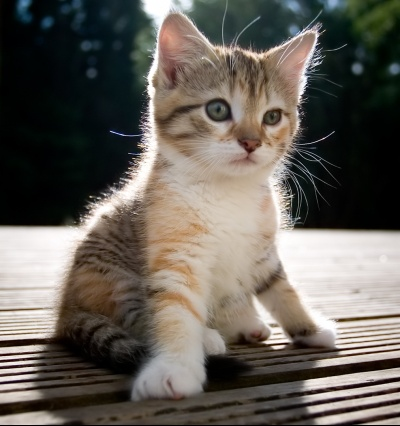
\includegraphics[scale=2]{chat.jpg}
\caption{L'image de départ}
\label{chat1}
\end{figure}




La figure \ref{chat2} représente l'image une fois que la compression a été appliquée avec un seuil assez petit pour garder la plupart des détails importants de l'image mais assez grand pour compresser les <<aplats>> de couleur, les ombres, etc. L'image compressée occupe 35\% de mémoire en moins par rapport à l'image de départ. Ce qui montre que la compression par ondelettes est plutôt efficace et que notre algorithme est fonctionnel.

\begin{figure}[!ht]
\centering
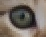
\includegraphics[scale=0.8]{chat_compress.jpg}
\caption{L'image compressée}
\label{chat2}
\end{figure}



Sur la figure \ref{chat3}, on peut voir l'image compressé avec le seuil maximal. Ici, tous les détails ont été éliminés. Cela revient simplement à diviser la résolution de l'image par deux.

\begin{figure}[!hb]
\centering
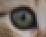
\includegraphics[scale=0.8]{chat_compress255.jpg}
\caption{L'image compressée à 100\%}
\label{chat3}
\end{figure}


\clearpage

\subsection{L'application graphique}

L'application graphique que nous avons créée permet plusieurs choses :

\begin{itemize}
\item Ouverture d'une image
\item Enregistrement d'une image
\item Affichage d'une image dans une fenêtre
\item Conversion d'une image en nuances de gris
\item Compression d'une image par deux méthodes
\item Réduction de la résolution d'une image de 50\%
\end{itemize}

La figure \ref{GUI} montre la fenêtre principale de l'application, avec une image en cours d'édition. L'interface est minimaliste, mais suffisante.



\begin{figure}[!hb]
\centering
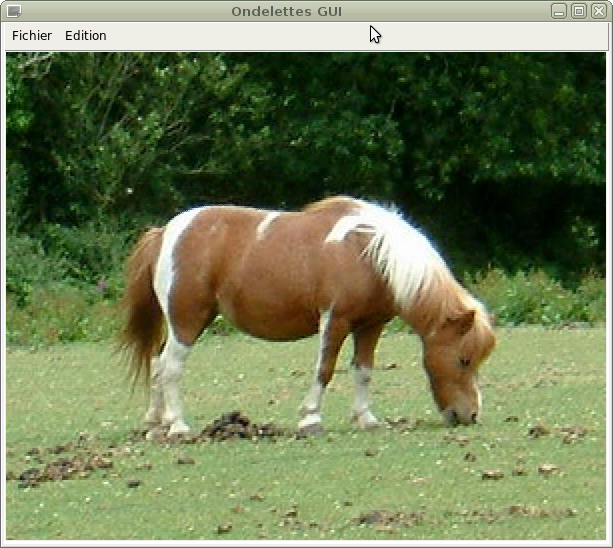
\includegraphics[scale=0.5]{OndelettesGUI.png}
\caption{Fenêtre principale de l'application}
\label{GUI}
\end{figure}


La figure \ref{GUI1} montre les menus de l'application, qui permettent de choisir entre toutes les actions décrites ci-dessus.

\begin{figure}[!ht]
\centering
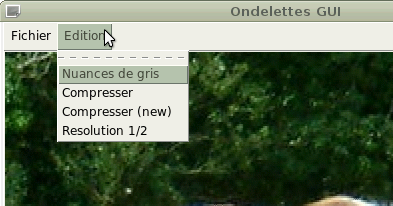
\includegraphics[scale=0.8]{OndelettesGUI1.png}
\caption{Menus de l'application}
\label{GUI1}
\end{figure}

La figure \ref{GUI2} montre le sélecteur de seuil, qui apparaît lorsqu'on choisit <<Compresser>> ou <<Compresser (new)>> dans les menus.

\begin{figure}[!hb]
\centering
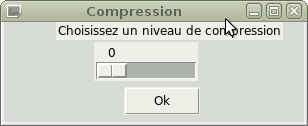
\includegraphics[scale=0.8]{Compression.png}
\caption{Le sélecteur de seuil de compression}
\label{GUI2}
\end{figure}


\cleardoublepage

\section{Description du code}

Ce qui suit est une description du code de tous nos programmes.

\subsection{Le fichier ondelettes.py }

Dans ce fichier, nous définissons des classes qui permettent le traitement des images. Il peut très bien être utilisé tout seul (sans l'interface graphique). 

\subsubsection{La classe Matrice }

Au lieu d'utiliser la classe Matrice du module @numpy@, nous avons préféré créer la notre. En effet, nous n'avons pas besoin de toutes les fonctions qu'elle offre. Aussi, nous voulions faire un maximum de choses nous-mêmes.

\paragraph{La fonction init }

Cette fonction prend en argument la taille de la matrice et le premier élément qu'elle doit contenir pour ensuite créer un tableau de tableaux contenant ce premier élément. Elle enregistre aussi les dimensions de la matrice dans l'objet créé.

\paragraph{La fonction transpose }

Comme son nom l'indique, elle transforme la matrice en sa transposée. Elle est utilisée lors de la transformation par ondelettes de Haar.

\paragraph{La fonction add}

Elle permet l'addition de matrices. La matrice sur laquelle est appelée la fonction est replacée par le résultat de l'addition. Elle n'est pas utilisée dans ce programme, mais pour que notre classe soit réutilisable dans d'autres projets, il fallait qu'elle soit créée.

\paragraph{La fonction multiply}

Cette fonction est analogue à la fonction @add@ pour la multiplication.

\paragraph{La fonction copy}

Cette fonction transorme la matrice en celle qui est passée en argument.

\paragraph{La fonction update}

Cette fonction met à jour les dimensions de la matrice si le tableau a changé de taille.

\paragraph{Les fonctions save et save1} 

Elles permettent de sauvegarder l'état de la matrice dans un tableau auxilliaire.

\paragraph{La fonction restore}

Elle remet en place le tableau sauvegardé par la fonction @save@.




\subsubsection{La classe MatriceImage}

Cette classe utilise la classe @Matrice@ pour stocker une image afin de pouvoir travailler dessus. Elle contient également des fonctions de compression et d'enregistrement.

\paragraph{La fonction init}

Cette fonction prend en argument l'emplacement d'une image et la charge à l'aide de PIL. Elle crée puis remplit une @Matrice@ avec les informations des pixels de l'image (cf. fonction @fill@).

\paragraph{La fonction fill}

Cette fonction stocke les pixels de l'image dans la @Matrice@.

\paragraph{Les fonctions grayscalemean et grayscalemeanmatrix}

Elles transforment l'image en nuances de gris en remplaçant chaque couleur de chaque pixel par la moyenne des trois composantes RGB du pixel.
@grayscalemean@ fait l'opération sur l'image directement alors que @grayscalemeanmatrix@ la fait sur la @Matrice@ de l'image.

\paragraph{Les fonctions getmatrixred, getmatrixgreen et getmatrixblue}

Créent des tableaux dans l'objet et les remplissent avec les composantes RGB (respectivement) de l'image. Cela permet de traiter chaque couleur séparément.

\paragraph{La fonction save}

Elle prend en argument une chaîne de caractère et sauvegarde l'image sous ce nom dans le dossier courant.

\paragraph{La fonction ondelette\_{}haar}

Cette fonction prend en argument un tableau de valeurs et le nombre de récursions qu'elle doit faire. Elle renvoie le tableau des coefficients d'approximation ainsi que le tableau des coefficients d'ondelette.

\paragraph{Les fonctions getcolonne et getligne}

Ces fonctions servent à récupérer une liste contenant les données d'une colonne/d'une ligne, pour pouvoir ensuite être traitées par la fonction ondelette\_{}haar.


\paragraph{La fonction setcolonne}

Elle permet de remettre une colonne dans une matrice après traitement.

\paragraph{Les fonctions apply\_{}haar\_{}lig et apply\_{}haar\_{}col}

Ces fonctions appliquent la transformation avec l'ondelette de haar à toutes les lignes/toutes les colonnes d'une matrice.

\paragraph{La fonction haar\_{}grayscale}

Cette fonction convertit une image en nuances de gris, puis applique la transformation par ondelettes sur l'image. Elle l'applique d'abord sur les lignes, puis transpose la @Matrice@, puis la réapplique sur les lignes.

\paragraph{La fonction update}

Elle est similaire à celle qui a été décrite plus haut.

\paragraph{La fonction create\_{}coef\_{}matrix}

Elle crée les tableaux nécessaires à la mise en mémoire des coefficients d'ondelette de chaque couleur.

\paragraph{La fonction haar}

Elle a le même effet que la fonction @haar\_{}grayscale@, mais elle s'applique aux 3 composantes de l'image.

\paragraph{La fonction makeimage}

Cette fonction crée une image à partir des matrices des coefficients d'approximation.

\paragraph{La fonction compression}

Cette fonction, une fois que les matrices de coefficients d'ondelette ont été créées, permet de supprimer les coefficients qui sont inférieurs au @epsilon@ passé en paramètre.

\paragraph{Les fonctions syntheseligne et synthesecolonnes}

Ces fonctions appliquent la transformation inverse à l'image, à partir des coefficients d'approximation et des coefficients d'ondelette qui ont été conservés par la fonction @compression@.

\paragraph{La fonction clearimage}

Elle supprime toutes les données d'une image en la remplissant d'une couleur définie.

\paragraph{La fonction fasthaar}

Cette fonction permet d'appliquer la transformation par ondelettes sans passer par les matrices. Pour cela elle prend tous les <<carrés>> de 4 pixels d'une image et leur applique la transformation et la compression. Elle est plus rapide que les autres fonctions, mais l'inconvénient est que la récursivité n'est pas permise. Elle est donc utilisée pour compresser légèrement une image. Les résulats restent tout de même impressionnant, puisqu'elle peut faire gagner jusqu'à 45\% d'espace en seulement quelques secondes.



\subsection{Le fichier ondelettesGUI.py}

Ce fichier est l'interface graphique du programme, qui requiert le fichier @ondelettes.py@ pour fonctionner. En effet, l'interface graphique n'est qu'une façade pour les fonctions qui ont été décrites plus haut.

\subsubsection{La classe Appli}

Cette classe représente la fenêtre principale de l'application.

\paragraph{La fonction init}

Cette fonction définit simplement l'instance de la fenêtre en appelant la fonction @initUI@ décrite plus bas.

\paragraph{La fonction initUI}

Cette fonction crée tous les éléments de la fenêtre (le titre et les menus, entre autres).

\paragraph{La fonction askopenfilename}

Cette fonction ouvre une boite de dialogue demandant quel fichier ouvrir. La boite de dialogue est incluse dans l'installation de Tkinter.
Une fois que le fichier a été choisi, la fonction crée la zone où l'image sera affichée.

\paragraph{La fonction asksaveasfilename}

Cette fonction ouvre une boite de dialogue demandant où enregistrer le fichier qui a été modifié.

\paragraph{Les fonctions askcompression et askcompression2}

Elles servent à ouvrir une boite de dialogue du type @DialogScale@ (défini plus bas) pour demander à l'utilisateur le seuil de compression à utiliser lors de l'appel des fonctions @compression@ ou @compression2@.


\paragraph{Les fonctions compression et compression2}

Ces fonctions utilisent respectivement les fonctions @haar@ et @fasthaar@ de @ondelettes.py@ pour réaliser la compression de l'image avec le seuil donné par les fonctions @askcompression@ et @askcompression2@. L'ancienne image est ensuite effacée de l'écran et la nouvelle est affichée grâce à @displayimage@;

\paragraph{La fonction grayscale}

Elle utilise les fonctions de @ondelettes.py@ pour convertir l'image en nuances de gris.

\paragraph{La fonction displayimage}

Elle crée une zone pour afficher la nouvelle image qui a été créée par compression, puis l'affiche dans cette zone.

\paragraph{La fonction onExit}

Elle est appelée lors de la fermeture de l'application et est là pour être sûr que tout est fermé correctement.



\subsubsection{La classe DialogScale}

C'est la classe qui définit la boîte de dialogue de compression (Fig.\ref{GUI2}). Elle est construite sur la même base de fenêtre que la classe @Appli@.

\paragraph{La fonction initUI}

Cette fonction crée le texte de la boîte de dialogue, le réglette qui permet de choisir la compression, et le bouton <<Ok>>.

\paragraph{La fonction onScale}

Elle est appelée lorsque l'utilisateur modifie la position de la réglette. Elle stocke la position de celle-ci en mémoire. 

\paragraph{La fonction ok}

Elle est appelée lorsque l'utilisateur clique sur le bouton <<ok>>. Elle sauvegarde la valeur de la position de la réglette, puis ferme la boîte de dialogue.

\subsubsection{La fonction main}

Elle crée simplement une instance de la classe @Appli@ et l'exécute.



\clearpage

\section{Annexes}

\subsection{Fichier ondelettes.py}
\lstinputlisting{ondelettes.py}

\subsection{Fichier ondelettesGUI.py}
\lstinputlisting{ondelettesGUI.py}

\section{Liens}

\begin{itemize}
\item Tous les fichiers .tex, .py de ce document : https://github.com/timosis/TIPE2013-2014

\item L'interpréteur Python : http://www.python.org/

\item La librairie PIL pour Python : http://www.pythonware.com/products/pil/

\item La licence GNU GPL : http://www.gnu.org/licenses/gpl-3.0.en.html


\item Source http://www.cmi.univ-mrs.fr/\textasciitilde{}melot/Master2/TPsignal\_PS.html
\end{itemize}
\end{document}
